\chapter{Experimental Setup}

\section{Pig Hearts}

In this study we used healthy and infarcted porcine hearts. The hearts were freshly excised, suspended in a plexiglass phantom filled with fluorinert (to eliminate artifacts) and placed in an MR head coil for ex vivo imaging. All DW-MR studies were performed on a dedicated 1.5T GE Signa Excite scanner using a custom FSE pulse sequence. We used the following MR parameters: TE = 35 ms, TR = 700 ms, echo train length = 2, b value = 0 for the unweighted MR images and b value = 500 s/mm2 when the 7 diffusion gradients were applied, respectively. We used a $256 \times 256$ k-space, FOV = 10-16 cm and a slice thickness of 1.2 mm, yielding a sub-millimetric voxel size. \\
From each heart, select samples containing an infarct were cut to align with the short-axis view of the MR images and prepared for histopathology to confirm the collagen deposition in the infarct area. \ref{fig:histology_pig_4} shows a histology image of a slide from an infarcted heart, with intact myocytes in the normal tissue and altered tissue microstructure in the infarcted zone. As depicted by the Masson Trichrome stain, the ischemic border zone (BZ) had collagen fibrils interdigitated between viable myocytes. In the dense scar area, necrotic myocytes were completely replaced by mature fibrosis (the final product of collagen degradation), resulting in the loss of myocardial anisotropy.\\\\\\

\begin{figure}[h!]
    \centering
    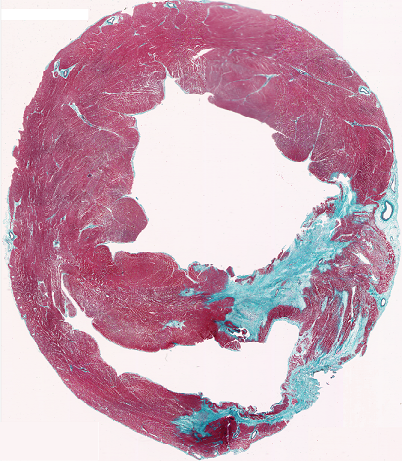
\includegraphics[width=\textwidth]{figures/histology_pig_4}
    \caption{Histology of a slice of infarcted heart nb 4}
    \label{fig:histology_pig_4}
\end{figure}

\section{Source of input data}

The data we have been using are DT-MRI of porcine hearts, both healthy for comparison and infarcted. We have had access to 10 hearts including 2 healthy. For every infarcted heart, the imaging process took place 6 weeks after infarct and histology was then done for most of the cases, which allows us to compare our observations to the ground truth.

\begin{center}
 \begin{tabular}{|c | c | c | c|} 
 \hline
 Heart & Region of infarct \\
 \hline
 2 & LCX \\ 
 \hline
 4 & LAD \\
 \hline
 5 & LCX \\
 \hline
 6 & ? \\
 \hline
 7 & ? \\ 
 \hline
 17 & ? \\
 \hline
 18 & ? \\
 \hline
 23 & ? \\
 \hline
 25 & Healthy \\
 \hline
 28 & ? \\
 \hline
\end{tabular}
\end{center}

\section{Quality of our data}

We will use for illustration purposes the hearts with the best quality and the least amount of noise, that is for the healthy heart number 5 and for the infarcted hearts 4 \& 7. \\
Due to the imaging technology used, and to the fact that a fairly low Tesla intensity was used to acquire this data (1.5T), a good amount of noise is present in the raw data. We have taken advantage of the knowledge on this noise (Rician noise) to apply non-local denoising strategies which are a bit expensive in time but can smooth rather efficiently and not by too much the data to be able to have a better readability of the fiber orientation without oversmoothing to prevent this strategy from smoothing even regions where the data is chaotic due to the infarct or proximity to the boundary more than because of noise issues.

\section{Usage of MedInria software to read the DICOMs}

We took the advantage of the MedInria tool to load the DICOM images, proceed the Rician denoising method and finally use their Diffusion Tensor Imaging tool to compute the value of the tensor matrix at each voxel location in the heart. \\
From the tensor matrices at every location, we were easily able to compute the fiber orientation at every location with a potential flip in the sense of the vector. Cylindrical consistency was used to enforce a consistent sense throughout the heart. \\
Once we have the fiber orientation at every voxel, we can use our previous work to compute the connection forms and get an approximative appreciation of the quality of the fitting, depending on hyper parameters that have to be fine tuned by mostly on the coherence of the underlying data.